
\eject{}
\section{Foreign, Partitioned, and Cursored Arrays}
\label{section:rich-structure}

A major advantage of the type-indexed approach is that it supports a richer variety of array representations, each supporting different usage patterns. In a perfect world one might hope for a single silver-bullet representation that magically does everything well. In the messier real world, it is a real step forward to express the cost model clearly but non-intrusively, as we show in this section.

\subsection{Representation Polymorphism and Foreign Arrays}
\label{section:ReprPoly}
\begin{figure}
\begin{small}
\begin{code}
data F  -- Type index for Foreign arrays.

instance Storable a => Source F a where
 data Array F sh e
   = AForeignPtr sh !Int !(ForeignPtr e)
  ...
instance Storable e => Target F e where
 data MVec F e = FPVec !Int !(ForeignPtr e)
 ...
\end{code}
\caption{Foreign Arrays}
\label{figure:ForeignArrays}
\end{small}
\end{figure}

The code needed to support foreign memory buffers is shown in Figure~\ref{figure:ForeignArrays}. With this representation we can construct an array \emph{directly into} a foreign buffer without going via the Haskell heap. This is achieved with the following function:
\par
\begin{small}
\begin{code}
 computeIntoIOP :: Load rs sh e
                => ForeignPtr e -> Array rs sh e -> IO ()
 computeIntoIOP !fptr !arr = loadP arr (FPVec 0 fptr)
\end{code}
\end{small} \par
Rather than returning the manifest array like @computeP@, this function takes the address of a foreign buffer and fills it by side effect in the @IO@ monad.

% -----------------------------------------------------------------------------
\subsection{Partitioned Arrays}
\label{section:Partitioned}
\label{section:Undefined}

\begin{figure}
\begin{small}
\begin{code}
data P r1 r2  -- Index constructor for partitioned arrays.

-- Source instance for (P r1 r2) -----------------------
instance (Source r1 e, Source r2 e)  
       => Source (P r1 r2) e where
 data Array (P r1 r2) sh e
   = APart { apExtent    :: sh
           , apHeadRange :: Range sh
           , apHead      :: Array r1 sh e
           , apTail      :: Array r2 sh e }
 index (APart _ r arr1 arr2) ix
   | rangeMatch r ix     = index arr1 ix
   | otherwise           = index arr2 ix
   
data Range sh
   = Range { rangeLow   :: sh, rangeHigh  :: sh
           , rangeMatch :: sh -> Bool }

-- The LoadRange class  --------------------------------
class (Source rs e, Shape sh) => LoadRange rs sh e where
 loadRangeP, loadRangeS 
    :: Target rt e
    => Array rs sh e -> MVec rt e -> Range sh -> IO ()

instance LoadRange D e where ...

-- Empty arrays ----------------------------------------
data X
instance Source X e where
  data Array X sh e = AUndefined sh
  index _ _         = error "element is undefined"
instance LoadRange X sh e where
  fillS _ _ = return ()
  fillP _ _ = return ()
\end{code}
\end{small}
\caption{Partitioned Arrays}
\label{figure:Partitioned}
\end{figure}

A \emph{partitioned array} consists of two neighbouring rectangular \emph{regions}, each represented by their own @Array@.  If these arrays are themselves partitioned, we can sub-divide an array into any number of regions.  Our primary use-case is to represent the result of a stencil convolution, where the element function that defines the inner region does not need to worry about what to do when applied close to the border of the array \cite{Lippmeier:Stencil}. 

The representation of partitioned arrays is shown in Figure~\ref{figure:Partitioned}. The @data@ declaration for @Array (P r1 r2)@ defines a partitioned array to consist of two sub-arrays (@apHead@ and @apTail@), together with a field, @apHeadRange@, that defines the range of indices covered by @apHead@.  Somewhat irregularly, the sub-arrays are indexed directly by the index of the outermost array, so the sub-arrays cover an index range that may not be zero-based.  To @index@ an element in a partitioned array, we use the @rangeMatch@ field of @apHeadRange@ to test whether its index is within the range of @apHead@ and if so index into @arr1@, otherwise we index into @arr2@.  The @Range@ type defines a rectangular range of elements between the two indices with type @sh@, and our @Load@ instance uses these two fields to compute starting and ending offsets during parallel computation:
\par
\begin{small}
\begin{code}
  instance (LoadRange r1 sh e, Load r2 sh e)
         => Load (P r1 r2) sh e where
   loadP (APart { apHeadRange = range
                , apHead = arr1,  apTail = arr2 }) mvec
    = do loadRangeP arr1 mvec range
         loadP      arr2 mvec 
\end{code}
\end{small}
%
The @Load@ class declaration was given in Figure~\ref{figure:Target}. The above instance uses the auxiliary class @LoadRange@ (Figure~\ref{figure:Partitioned}), which is just like @Load@, except that it only computes and writes elements in a specified @Range@. Since @apHeadRange@ only describes @apHead@, we use @loadRangeP@ for @apHead@, and @loadP@ for @apTail@. When we reach the right-most array (at the end of the @apTail@ chain) we have no explicit description of the range of indices covered. In this case we use an empty array with type index @X@ (see Figure~\ref{figure:Partitioned}). Thus a typical partitioned array might have a type like @PD5@ in Figure~\ref{figure:Cursored}; note that @X@ terminates this ``list'' of partitions. 

However, the critical point is this: \emph{the @loadP@ instance for partitioned arrays can be completely unfolded by the GHC simplifier at compile-time}. For example, given the following call:
%
\begin{small}
\begin{code}
   loadP (arr :: Array (P D (P D X)) DIM2 Float)
\end{code}
\end{small}
%
GHC can inline the code for @loadP@ at type @(P D (P D X))@, which produces code with a call to @loadP@ at type @(P D X)@. GHC can inline that too, yielding code that calls @loadP@ at type @X@, and that can be inlined trivially.  The result is a sequence of two calls to @loadRangeP@, each at type @D@:
\par
\begin{small}
\begin{code}
  case arr   of { APart _  range1 arr11 arr12 ->
  case arr12 of { APart _  range2 arr21 _     ->
  do loadRangeP arr11 mvec range1
     loadRangeP arr21 mvec range2
     return ()  }}                 -- loadP at X 
\end{code}
\end{small}
%
Now GHC can inline the two calls to @loadRangeP@ at type @D@. We end up with a sequence of two loops, each executed in parallel.

This kind of inlining is guaranteed not to diverge, because the type of @arr12@ becomes smaller in each recursive
call, providing a structural termination condition for @loadP@. This is similar to the termination conditions used by
theorem proving languages such as Coq~\cite{Coq} and Agda~\cite{Norell:Agda}. The use of type indices to guide the compiler solves the code explosion problem discussed in \S\ref{section:Explosion}, as our array filling functions are now unfolded only as many times as needed for the source array.


% -----------------------------------------------------------------------------
\subsection{Structure Preserving Maps}
\label{section:Structured}

\begin{figure}
\begin{small}
\begin{code}
class Source r a => Structured r a where
  type TR r
  smap     :: Shape sh 
           => (a -> b) 
           -> Array r sh a -> Array (TR r) sh b

  szipWith :: (Shape sh, Source r c)
           => (c -> a -> b) 
           -> Array r0 sh c  -> Array r sh a
           -> Array (TR r) sh b

instance Vector.Unbox a => Structured U a where
  type TR U = D
  smap      = map
  szipWith  = zipWith

instance (Structured r1 a, Structured r2 a)
       => Structured (P r1 r2) a where
  type TR (P r1 r2) = P (TR r1) (TR r2)

  smap f (APart sh range arr1 arr2)
        = APart sh range (smap f arr1) (smap f arr2)

  szipWith f arr1 (APart sh range arr21 arr22)
        = APart sh range (szipWith f arr1 arr21)
                         (szipWith f arr1 arr22)
\end{code}
\end{small}
\caption{Structured Maps}
\label{figure:Structured}
\end{figure}

Say we have @arr :: Array (P D (P D X)) DIM2 Float@. As we saw at the end of \S\ref{section:Partitioned}, the application @loadP arr@ will compile to two beautiful loops, one for each partition. However, suppose we also map a function across every element before loading from it, like with @(loadP (map negate arr))@. Referring to Figure~\ref{figure:map}, we see that @map@ always produces a delayed result, with type index @D@. The @loadP@ only sees a delayed array, and will generate a single loop in which each indexing operation performs a conditional test on @arr@ to determine which partition to use. Disaster: this is \emph{slower} than not having partitioned arrays in the first place.

What we want is for @map@ to be \emph{structure-preserving}: given a partitioned array, it should produce a partitioned array. However @map@ should not \emph{always} produce an array with the same representation as its input. Given a manifest array, @map@ should produce a delayed array. In short, \emph{the appropriate representation of @map@'s result is a function of the representation of its input}.  This is just what type functions are for!

Figure~\ref{figure:Structured} implements this idea. We use a new class @Structured@, whose methods are @smap@ and @szipWith@. The class has an associated type @TR@ (short for Target Representation), which computes the result representation from its argument. We can see a use of @TR@ in the type of @smap@. 

The @U@ instance of @Structured@ is simple, we just use the default @map@ implementation from Figure~\ref{figure:map}. The @(P r1 r2)@ instance from Figure~\ref{figure:Structured} is more interesting, as it preserves the partitioning structure of the source array.

Continuing on to @szipWith@, note that its type is right biased. The structure of its result is taken from the structure of the second array argument, ignoring that of the first. Preserving the partitioning of \emph{both} source arrays would be significantly more complicated. For example:
%
\begin{center}
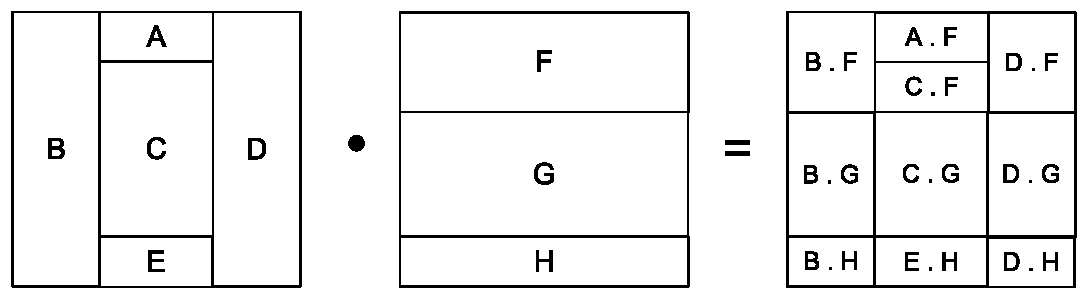
\includegraphics[scale=0.35]{figs/guiding-zipwith-partitions}
\end{center}
%
The number of partitions in the result depends on the number of partitions in the input arrays, which is a static property, as well as the \emph{sizes} of those partitions, which can be a dynamic property.

Repa~3 includes the original @zipWith@ as well as our new @szipWith@ function. With plain @zipWith@, if the overall shape of the source arrays is different, then the shape of the result is their intersection. Performing this intersection is straightforward when there is no internal structure to worry about. In contrast, @szipWith@  preserves the structure of the second source array, but the overall shape of both source arrays must match. 



% -----------------------------------------------------------------------------
\subsection{Cursored Arrays}
\label{section:Cursored}

\begin{figure}
\begin{small}
\begin{code}
data C   -- The type index for cursored arrays.

instance Source C sh a where
  data Array C sh e
     = forall cursor. ACursored
     { cursoredExtent :: sh 
     , makeCursor     :: sh -> cursor
     , shiftCursor    :: sh -> cursor -> cursor
     , loadCursor     :: cursor -> e }
  extent (ACursored ex _     _ _)     = ex
  index  (ACursored _  makec _ loadc) = loadc . makec
  linearIndex (ACursored sh makec _ loadc)
         = loadc . makec . fromIndex sh

instance Load C DIM2 e where
 loadP (ACursored (DIM2 w h) makec shiftc loadc) marr
  = fillCursoredBlock2P ...
        
type PD5 = P C (P D (P D (P D (P D X))))
mapStencil2 :: Source r sh a 
  => Boundary a     -> Stencil DIM2 a
  -> Array r DIM2 a -> Array PD5 DIM2 a
\end{code}
\end{small}
\caption{Cursored Arrays}
\label{figure:Cursored}
\end{figure}

The cursored arrays of \cite{Lippmeier:Stencil} are used to optimise stencil convolutions, by sharing intermediate values between the computation of adjacent pixels. Figure~\ref{figure:Cursored} contains the definition of cursored arrays using our new type-indexed framework. The @Array@ declaration in Figure~\ref{figure:Cursored} takes the role of the @Generator@ from Repa~2, with the role of @makeCursor@, @shiftCursor@ and so on being as per \cite{Lippmeier:Stencil}. 

The definition of @fillCursoredBlock2P@ in the @Load@ instance of Figure~\ref{figure:Cursored} is as per \cite{Lippmeier:Stencil}. As discussed there, its definition contains loops that have been hand-specialised with the unroll-and-jam transformation  \cite{Carr:unroll-and-jam} to separate array reads from array writes. This in turn enables LLVM's global value numbering transformation \cite{Rosen:global-value-nubering}, which recovers sharing of intermediate results between the computation of successive array elements. To improve cache performance, these loops also traverse the source and result arrays in column-wise order, as per the diagram in \S\ref{section:Interleaved}. This means that @fillCursoredBlock2P@ is specialised for arrays of rank-2, hence the @DIM2@ constraint in the @Load@ instance it is used in. 

The @mapStencil2@ function takes a stencil definition, a source array, a description of what to do at the boundary; and produces a partitioned array. This function is also specialised to rank-2 arrays, so the result is split into five partitions, one for inner region and one for each of the four borders. As the use of cursored arrays tends to increase the size of the intermediate code due to loop unrolling, we used a Cursored (@C@) array for the inner region only, defining the borders in terms of Delayed (@D@) arrays. The runtime cost of computing the border regions is typically only a tiny fraction of the cost of computing the internal region, and using delayed arrays for the borders keeps the compile-times and resulting executable size down.
